\documentclass{beamer}
\usetheme{}
\usecolortheme{dolphin}           
\useinnertheme{circles}
\setbeamertemplate{itemize items}[default]
\setbeamertemplate{enumerate items}[default]
\usepackage[T1]{fontenc}
\usepackage[utf8]{inputenc}
\usepackage{lmodern}
\usepackage{amsmath}
\usepackage{booktabs} 
\usepackage{graphicx}        
\usepackage{array}
\usepackage{color}
\makeatletter
\def\zapcolorreset{\let\reset@color\relax\ignorespaces}
\def\colorrows#1{\noalign{\aftergroup\zapcolorreset#1}\ignorespaces}
\makeatother
\graphicspath{{/home/swl/Dropbox/ucd/advanced_macro/figures/}} 
\setbeamertemplate{navigation symbols}{}
\setbeamertemplate{footline}[frame number]

%--------------------------------------
\title{Banking \& risk}
\author{School of Economics, University College Dublin}
\date{Spring 2018}
\begin{document}

%--------------------------------------
\begin{frame}
 \titlepage
\end{frame}
%--------------------------------------

%--------------------------------------
\begin{frame}
 Recall interest rate equation from NK model
  \begin{align} 
  i_t=r_t^n+ \phi_{\pi}\pi_t+\phi_xx_t 
\end{align}
\medskip
$i_t$ is a specific interest rate
\begin{itemize}
  \item Short-term risk-free overnight rate that banks charge each other
  \item Quite different from consumer interest rates
\end{itemize}
\medskip
To understand consumer interest rates need to understand risk involved with consumer lending. 
\end{frame}
%--------------------------------------

%--------------------------------------
\begin{frame}
 Suppose investor can choose between following two assets  
\begin{enumerate}
  \item Risk-free bond with interest rate $r$
  \item Loan with interest rate $R$ and probability of default $p$
  \begin{itemize}
    \item Return of $R$ with probability $1-p$
    \item Return of -1 (losing all your money) with probability $p$
  \end{itemize}
\end{enumerate}
\end{frame}
%--------------------------------------

%--------------------------------------
\begin{frame}
  Expected return on loan
  \begin{align}
   R(1-p)-p\\ \nonumber
    R-Rp-p\\ \nonumber
    R-p
\end{align}
 For same expecter return, interest $r$ needs to be 
\begin{align}
  r &= R-p\\ \nonumber
  r+p &=R
\end{align}
\end{frame}
%--------------------------------------

%--------------------------------------
\begin{frame}
 For loan with collateral, default return:
\begin{align}
  c-1<0  
\end{align}
\medskip
Eq.3 becomes
\begin{align}
  R=r+(1-c)p  
\end{align}
 \medskip 
 \begin{enumerate}
   \item Collateralised loans have lower interest rates
   \item Interest rate depends on type of collateral
 \end{enumerate}
\end{frame}
%--------------------------------------

%--------------------------------------
\begin{frame}
  \begin{figure}
    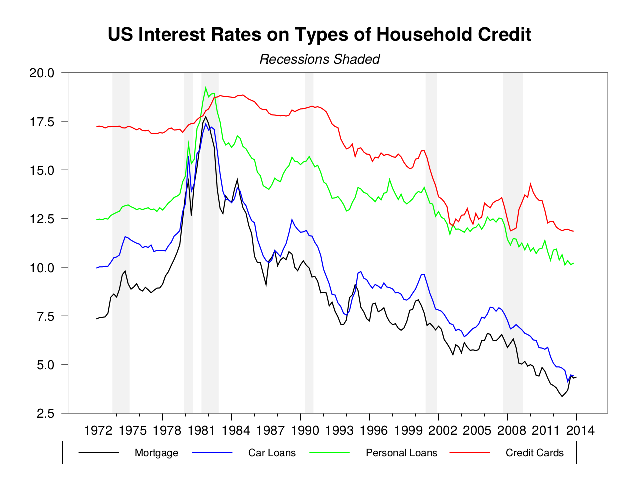
\includegraphics{us_interest_rates.eps}
  \end{figure}
\end{frame}
%--------------------------------------

%--------------------------------------
\begin{frame}
  \begin{figure}
    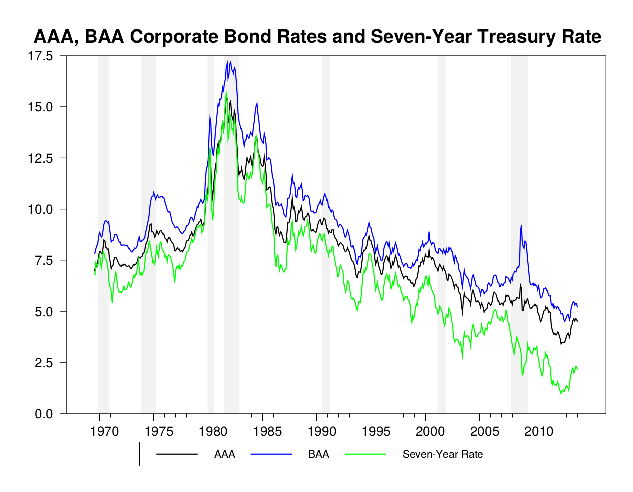
\includegraphics{bond_rates.eps}
  \end{figure}
\end{frame}
%--------------------------------------

%--------------------------------------
\begin{frame}
  \begin{figure}
    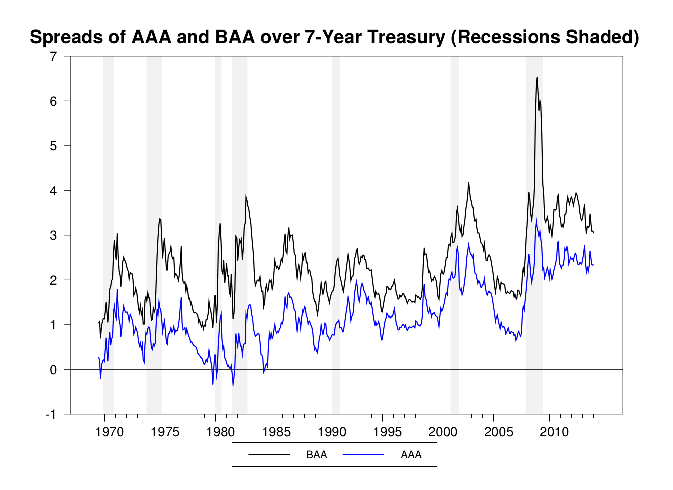
\includegraphics{bond_rates2.eps}
  \end{figure}
\end{frame}
%--------------------------------------

%--------------------------------------
\begin{frame}
 \textbf{Default risk and collateral}  
\begin{enumerate}
  \item Interest rate affected by value of collateral
  \item Value of assets fluctuate with state of economy
\end{enumerate}
 \medskip
 \text{Financial accelerator}: mechanisms by which financial sector can propagate business cycle shocks 
 \begin{itemize}
   \item Recession-causing shock will increase interest rate spreads which will worsen the recession
 \end{itemize}
\end{frame}
%--------------------------------------

%--------------------------------------
\begin{frame}
\textbf{Bernanke, Gertler \& Gilchrist} (1999) \\
  Demand
\begin{align}
  y_t &= \frac{C}{Y}c_t + \frac{I}{Y}inv_t + \frac{G}{Y}g_t + \frac{C^e}{Y}c^e_t+...\\
  c_t &= -\sigma r_{t+1} + E_tc_{t+1}\\
  c^e_t &= \frac{1-\phi}{\phi}n_{t+1}\\
  q_t &= \phi(i_t-k_t)  \\
  E_tr_{kt+1} &= (1-\rho)E_t(p_{wt+1}-p_{t-1} + y_{t-1} \\ \nonumber &- k_{t+1}) + \rho E_tq_{t+1} -q_t\\
  E_tr_{kt+1} - r_{t+1} &= -v(n_t -q_t -k_{t+1})  
\end{align}
\end{frame}
%--------------------------------------

%--------------------------------------
\begin{frame}
  Supply
\begin{align}
  y_t &= a_t + \alpha k_t + (1-\alpha)l_t\\
  y_t-l_t &= \mu_t + \gamma_l l_t + c_t\\
  \pi_t &= \kappa (p_{wt}-p_t) + \beta E_t \pi_{t+1}
\end{align}
\end{frame}
%--------------------------------------

%--------------------------------------
\begin{frame}
  The evolution of the state variable 
\begin{align}
  k_{t+1} &= \delta inv_t + (1-\delta)k_t\\
  n_t &= \frac{\theta RK}{N}[r_ t^k - r_t] + \theta R(r_t+n_{t-1})\\
  r_t &= i_{t-1} - \pi_{t-1}
\end{align}
\medskip
Monetary policy rule is given by
\begin{align}
  i_t &= \rho i_{t-1} + (1-\rho)[\gamma_{\pi}\pi_t + \gamma_y(y_t - y_t^n)]+ \epsilon_t^{rn}\\
  i_t &= r_{t+1} - E_t\pi_{t+1}
\end{align}
\end{frame}
%--------------------------------------

%--------------------------------------
\begin{frame}
 \begin{figure}
   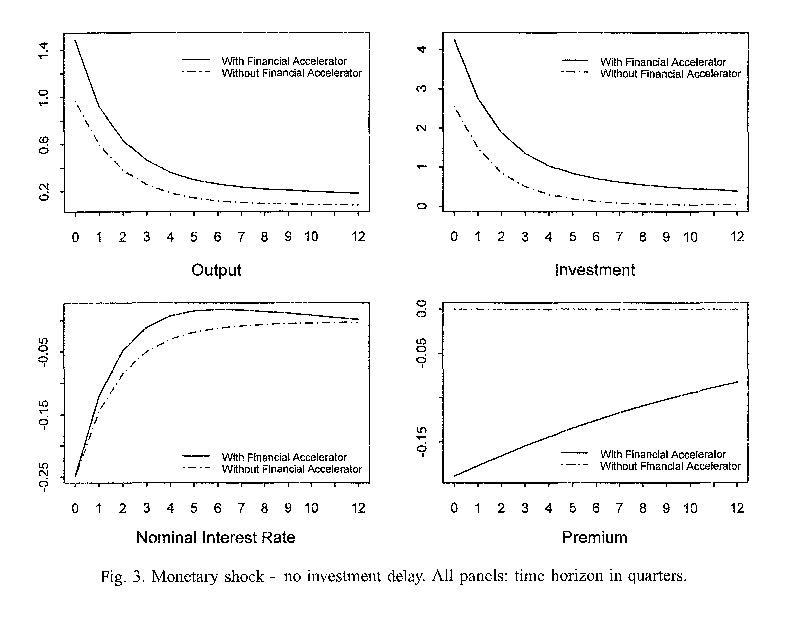
\includegraphics[scale=.8]{bernanke.eps}
 \end{figure}  
\end{frame}
%--------------------------------------

%--------------------------------------
\begin{frame}
 \begin{figure}
   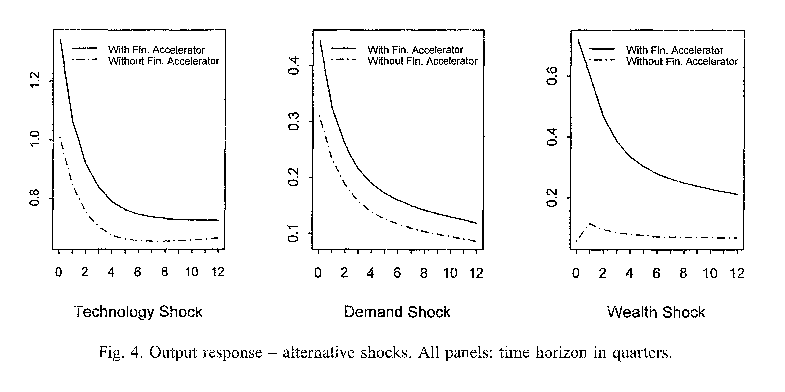
\includegraphics[scale=.8]{bernanke2.eps}
 \end{figure}  
\end{frame}
%--------------------------------------

%--------------------------------------
\begin{frame}
 \begin{figure}
   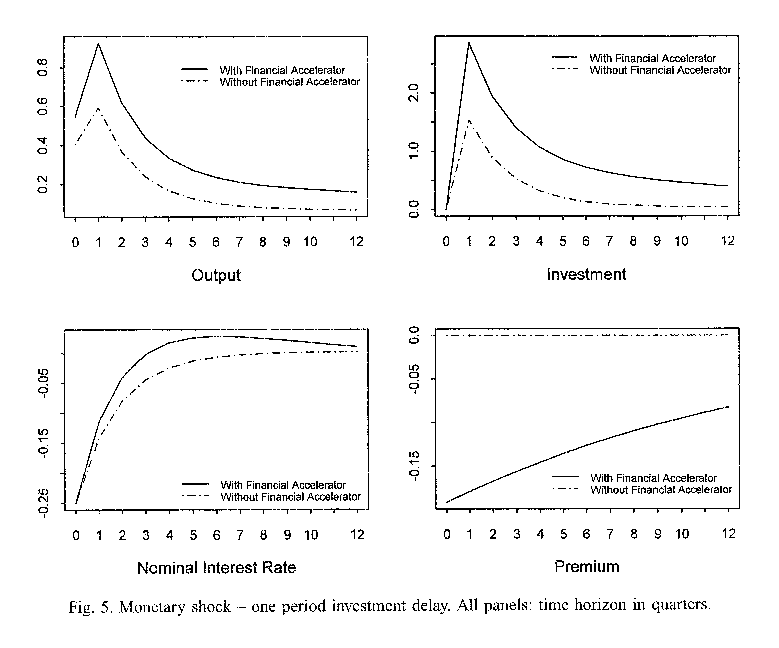
\includegraphics[scale=.8]{bernanke3.eps}
 \end{figure}  
\end{frame}
%--------------------------------------

%--------------------------------------
\begin{frame}
Borrowers with higher risk pay higher interest rates.
\begin{itemize}
  \item Assumption: for each risk level, someone willing to lend at high enough rates  
\end{itemize}
\medskip
 Credit suppliers can refuse to make a loan, rather than trying to balance the loss by raising the interest rate: \textbf{credit rationing}
\begin{quote}
  Lenders provide a smaller amount of loans than is demanded at the market interest rate.
\end{quote}
\end{frame}
%--------------------------------------

%--------------------------------------
\begin{frame}
 Asymmetric information in credit market:
\begin{itemize}
  \item Banks can't always tell good borrowers from bad
  \item From bank's point of view borrowers worsen as interest rates increase
\end{itemize}
  \medskip
  Credit rationing can be quite severe, turning down credit-worthy borrowers
\end{frame}
%--------------------------------------

%--------------------------------------
\begin{frame}
 \textbf{Stiglitz \& Weiss} (1981); Suppose number of borrowers each with a project to undertake
\begin{enumerate}
  \item All borrowers look to borrow $B$ and put up collateral $C$
  \item Projects deliver a sum of $R$  
  \item Interest rate on bank loans $r$ is determined endogenously
\end{enumerate}
\end{frame}
%--------------------------------------

%--------------------------------------
\begin{frame} 
 Return $R$ is uncertain
 \begin{itemize}
   \item Outcome distribution varies across borrowers 
 \end{itemize}
 \medskip
 Return distribution type $\theta$ borrowers 
 \begin{align}
   f(R,\theta)
 \end{align}
 \medskip
 Distribution mean identical across borrowers, but greater $\theta$ values correspond to greater riskiness
 \begin{itemize}
   \item High values of $\theta$ induce a mean-preserving spread in the distribution of projected payoffs
   \item Borrowers are observably identical to banks: don't observe an individual's value of $\theta$
 \end{itemize}
\end{frame}
%--------------------------------------

%--------------------------------------
\begin{frame}
  \begin{figure}
    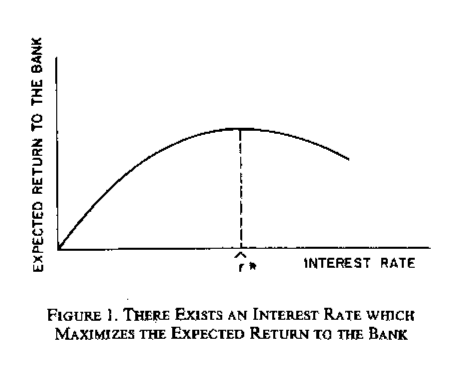
\includegraphics{stiglitz_weiss1.eps}
  \end{figure}
\end{frame}
%--------------------------------------

%--------------------------------------
\begin{frame}
 Mechanism: bank sets $r$ which might affect risk of loan through
\begin{enumerate}
  \item \textbf{Adverse selection}: Sorting potential borrowers
  \item \textbf{Moral hazard}: Affecting the actions of the borrowers
\end{enumerate}
\end{frame}
%--------------------------------------

%--------------------------------------
\begin{frame}
 \textbf{Default} 
\begin{align}
  C+R\leq B(1+r)
\end{align}
\medskip
$B$, amount borrowed\\
$C$, collateral
\end{frame}
%--------------------------------------

%--------------------------------------
\begin{frame}
 \textbf{Returns}\\
 \medskip
 For firm $\pi(R,r)$ 
\begin{align}
  \pi(R,r)=Max(R-(1+r)B;-C)
\end{align}
\medskip
For bank
\begin{align}
  \rho(R,r)=min(R+C;B(1+r))
\end{align}
\end{frame}
%--------------------------------------

%--------------------------------------
\begin{frame}
The worst a firm can do is default on the loan and lose the collateral when the project has a bad return
\begin{itemize}
  \item After that the return increases one for one with outcome $R$
  \item Return depends negatively on borrowing rate $r$
  \item Not all firms decide to go ahead and borrow as not all firms have a positive expected value.
\end{itemize}
\end{frame}
%--------------------------------------

%--------------------------------------
\begin{frame}
Firm borrows if
\begin{align}
  \mathbb{E}[\pi(R,r)]=\int_0^{\infty} \pi(R,r)f(R,\theta)dR>0
\end{align}
\medskip
Main question is how 
\begin{align}
  \mathbb{E}[\pi(R,r)]
\end{align}
\medskip
varies with type $\theta$
\end{frame}
%--------------------------------------

%--------------------------------------
\begin{frame}
\textbf{Borrower pool}: Decide to borrow if
\begin{align}
  \theta > \hat{\theta}(r)
\end{align}
\medskip
From utility theory;
\begin{itemize}
  \item If $U(C)$ is concave: mean-preserving spread in $C$ distribution reduces expected utility because people are risk averse
\end{itemize}
\medskip
In this case outcome is a convex function of $R$, so more uncertainty increases the expected return. 
\begin{itemize}
  \item Bad case:outcome still $−C$ but increased risk raises the chance of a really good outcome.
\end{itemize}
\end{frame}
%--------------------------------------

%--------------------------------------
\begin{frame}
 How does $r$ increase affect loan demand?  
\begin{itemize}
  \item Project returns depend negatively on $r$: increase in $r$ reduces everyone's expected project returns  
  \item Expected project returns depend positively on $\theta$: some firms still have positive expected value for
    going ahead with borrowing and doing the project
  \item Increase in $r$ raises the cut-off $\hat{\theta}(r)$ for potential borrowers
\end{itemize}
\medskip
 Interest rate increases; borrowers pool changes consisting of more risky project (adverse selection)
 \begin{itemize}
   \item Moral hazard problem: risk-neutral investors prefer project with higher bankruptcy probability
 \end{itemize}
\end{frame}
%--------------------------------------

%--------------------------------------
\begin{frame}
\textbf{Bank pay off}
\begin{align}
  Min(R+C;(1+r)B)
\end{align}
 If bank knows it is lending to type $\theta$; expected return
\begin{align}
  \rho(\theta,r)=\int_0^{\infty}[Min(R+C;(1+r)B)]f(R,\theta)dR
\end{align}
 \medskip
 Bank's pay off concave function of $R$: increases in $\theta$ reduces bank's expected return.
\end{frame}
%--------------------------------------

%--------------------------------------
\begin{frame}
 \begin{enumerate}
   \item Best case: bank gets principal and interest
   \item Worst case: only get collateral
 \end{enumerate}
 \medskip
 More risk is bad, but bank cannot tell if borrowers is risky
 \begin{itemize}
   \item Expected payoff can be calculated averaging across all types that look for loans at interest rate $r$
 \end{itemize}
\begin{align}
  \mathbb{E}[\rho(\theta,r)]=\frac{\int_{\hat{\theta}(r)}^{\infty}\rho(\theta,r)dG(\theta)}{1-G(\hat{\theta})}
\end{align}
\end{frame}
%--------------------------------------

%--------------------------------------
\begin{frame}
  \begin{figure}
    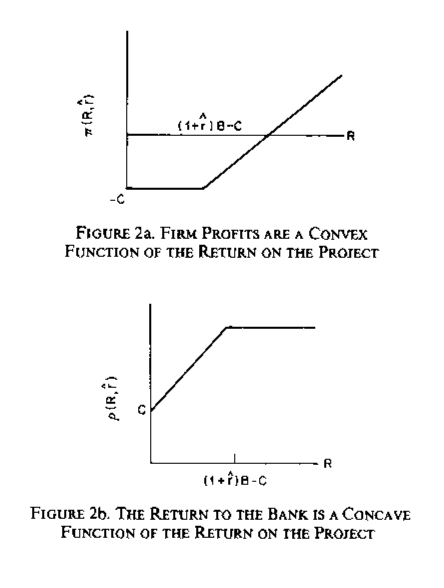
\includegraphics{stiglitz_weiss2.eps}
  \end{figure}
\end{frame}
%--------------------------------------

%--------------------------------------
\begin{frame}
 $r$ increase has two effects on bank's pay off 
\begin{enumerate}
  \item +ve: higher interest revenues from each project that pays off
  \item -ve: adverse selection.   
\end{enumerate}
At some point second effect dominates: bank profits rise as the interest rate goes up, reach a maximum and then decline
\end{frame}
%--------------------------------------

%--------------------------------------
\begin{frame} 
 \textbf{Borrower type}
 \begin{enumerate}
   \item Low risk
   \item High risk
 \end{enumerate}
 Profits drop at point where low-risk types drop out
 \begin{itemize}
   \item Continuous number of types: interest rate $r^*$, which is consistent with maximum profit level
   \item Assume that loan supply depends positively on the expected pay off
 \end{itemize} 
\end{frame}
%--------------------------------------

%--------------------------------------
\begin{frame}
Problem: banks cannot simply choose $r^*$
 \begin{itemize}
   \item No equilibrium if there is not sufficient demand
   \item Banks would chase consumers offering them $r^*$ and lots of people would be turning them down
 \end{itemize}
\end{frame}
%--------------------------------------

%--------------------------------------
\begin{frame}
 Equilibrium outcome determined by supply/demand interaction
\begin{enumerate}
  \item Low loan demand
  \begin{itemize}
    \item Loan demand curve intersects loan supply curve below $r^*$. 
    \item Market functions normally: all who request a loan receive one
\end{itemize}
\medskip
  \item High loan demand
  \begin{itemize}
    \item Loan demand and supply curves do not intersect: bank pick optimal interest rate $r^*$    
    \item Credit rationing: More demand than banks are willing to supply
  \end{itemize}
\end{enumerate}
\end{frame}
%--------------------------------------


%--------------------------------------
\begin{frame}
  \begin{figure}
    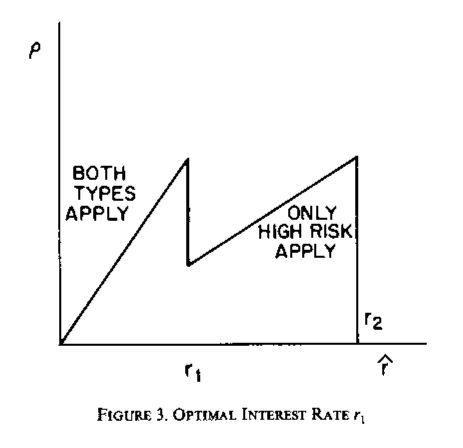
\includegraphics{stiglitz_weiss3.eps}
  \end{figure}
\end{frame}
%--------------------------------------

%--------------------------------------
\begin{frame}
 Examples sovereign defaults:\\
 \medskip
 Early 1800s: number of countries after the Napoleonic Wars, e.g. Denmark, France, the Netherlands, and Sweden\\
 1875: Ottoman Empire\\
 1932: Germany\\
 1982: Mexico\\
 1998: Russia\\
 2006: Zimbabwe\\
 1982, 1989, 2001: Argentina\\
 1826, 1843, 1860, 1894, 1932, 2015: Greece
\end{frame}
%--------------------------------------

%--------------------------------------
\begin{frame}
  \begin{figure}
      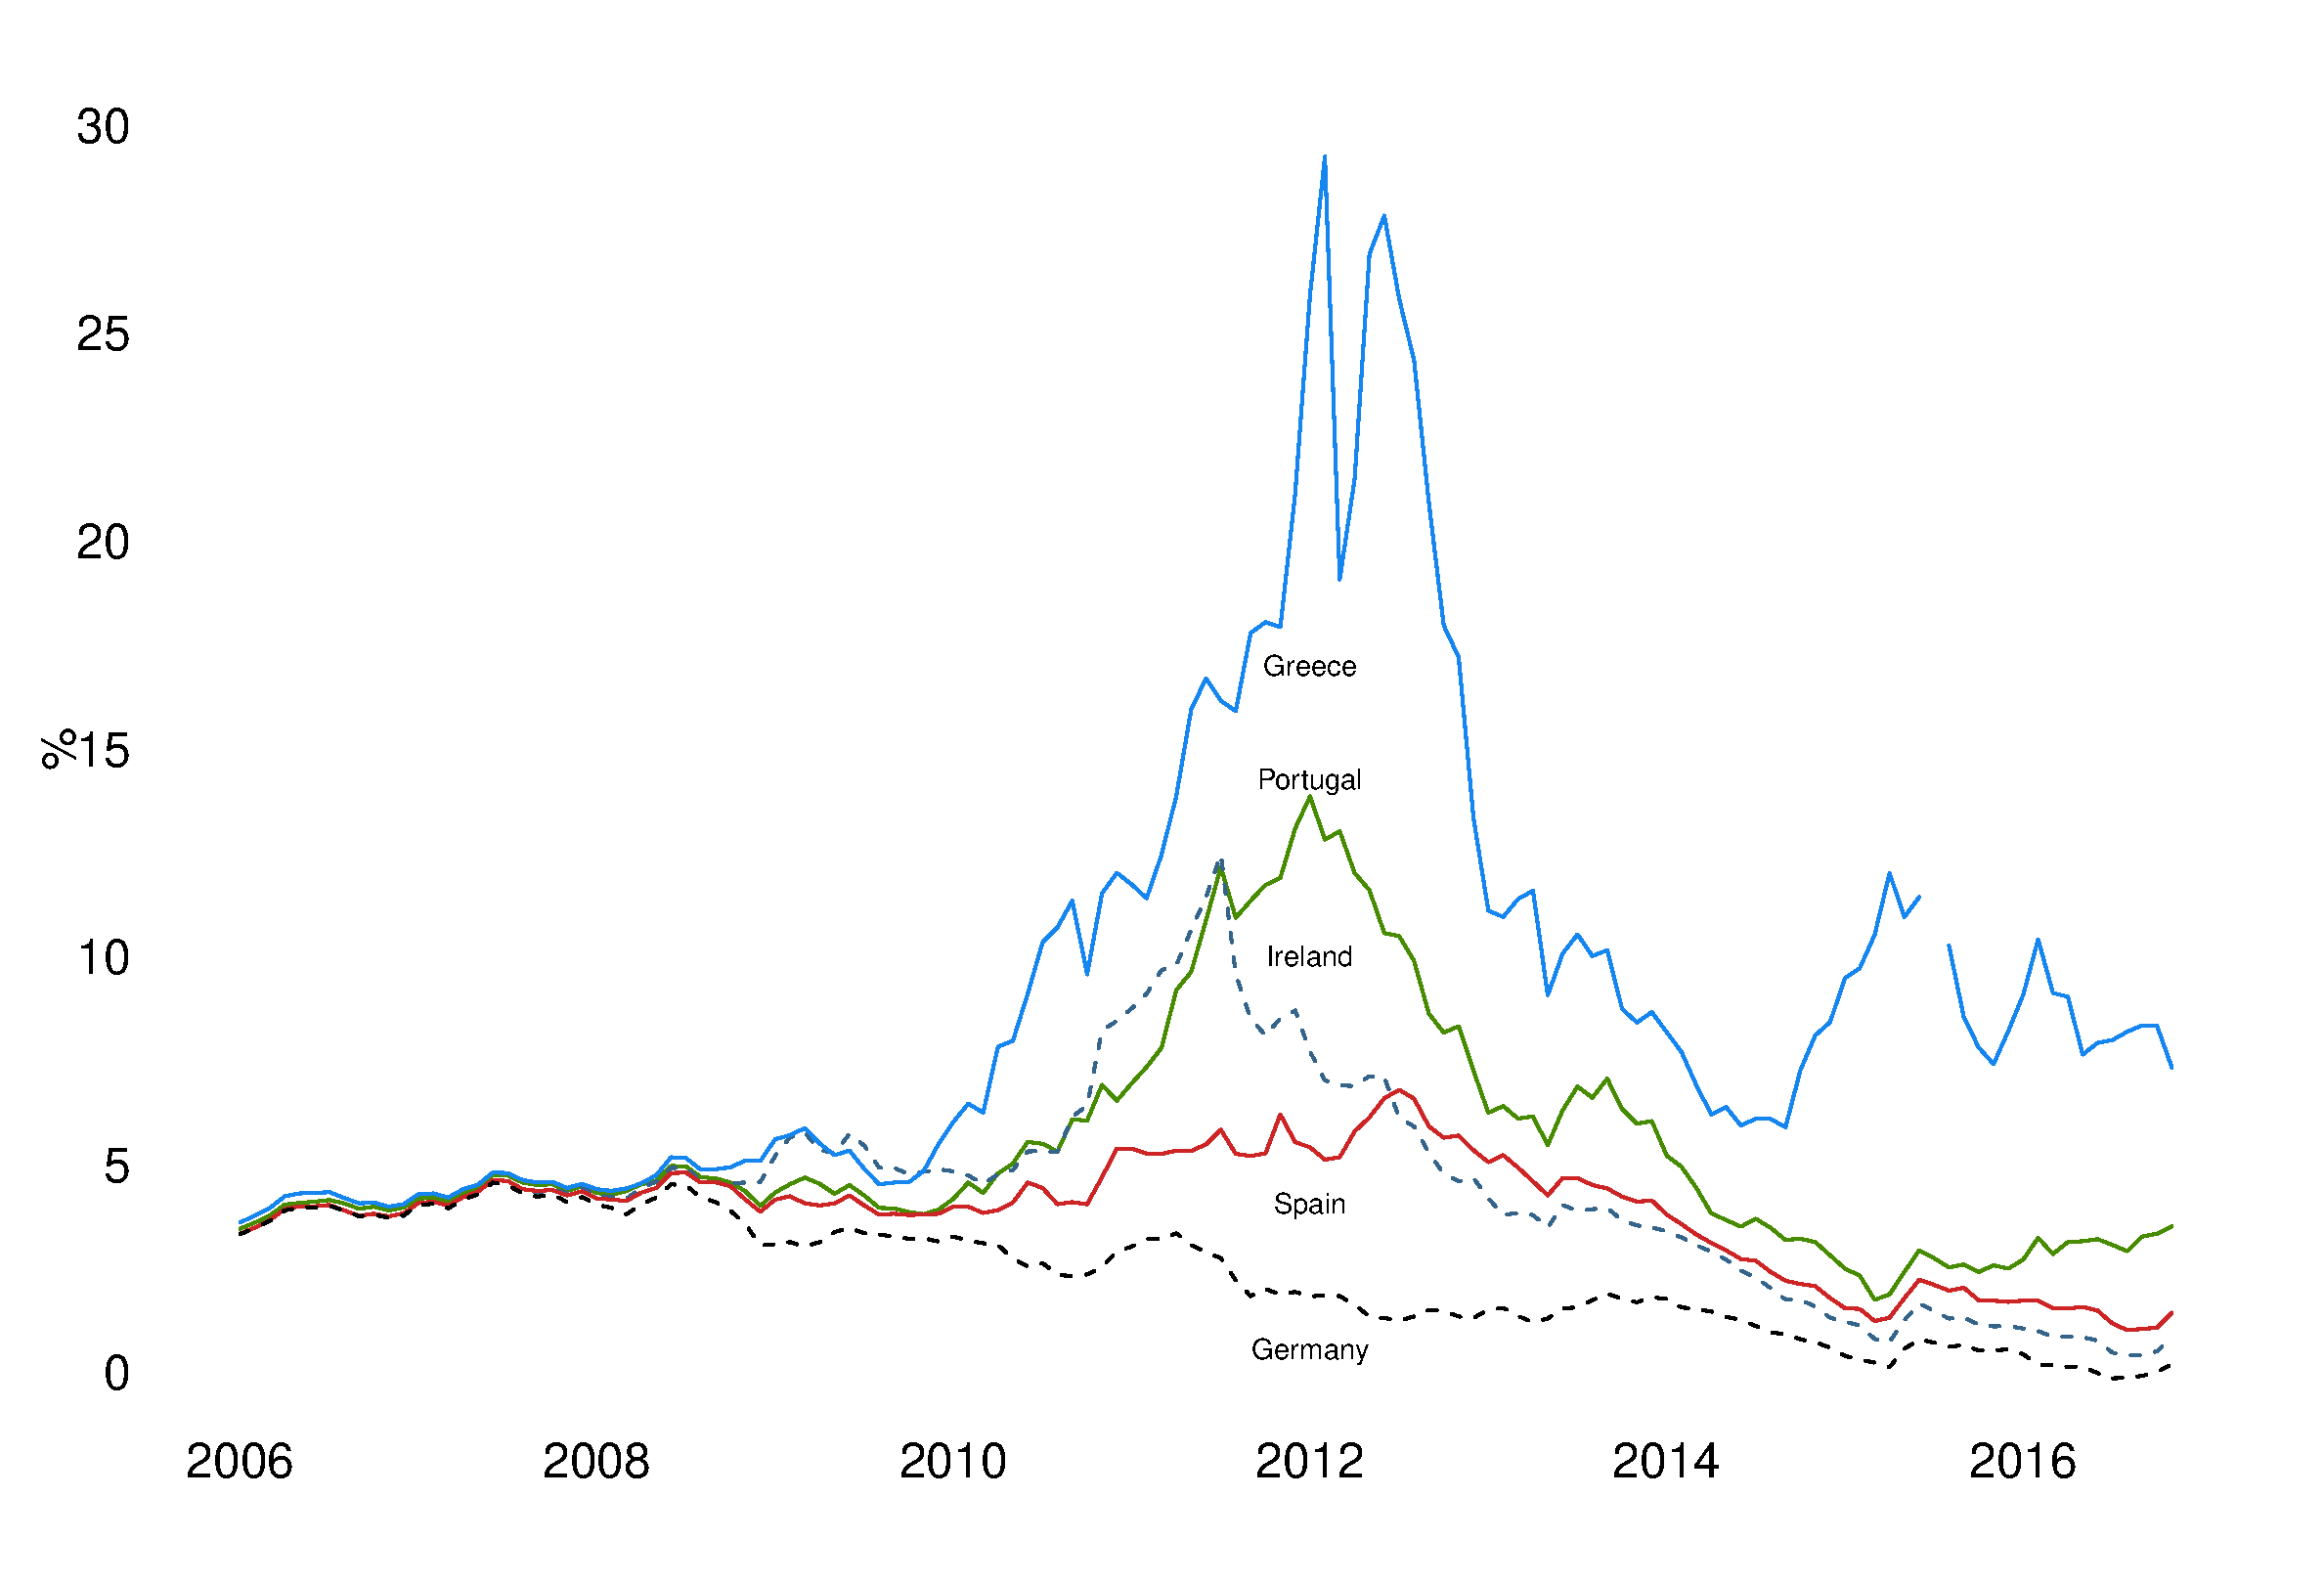
\includegraphics[scale=.3]{bonds.eps}
    \end{figure}  
\end{frame}
%--------------------------------------

%--------------------------------------
\begin{frame}
  Consider country has $P(default)=0.1$ over next year; leading to 50\% default on outstanding debt
  \begin{itemize}
    \item Country needs to pay 5\% premium on debt relative to safe assets
  \end{itemize}
  \medskip
  Premium imposes additional burden on government
  \begin{itemize}
    \item Interest costs rise above the funds that country can access to pay off the interest payments
    \item Alternatively the country's GDP could expand in order to keep debt stable
  \end{itemize}
  Market for government bonds might cease to operate as the country is deemed not credit-worthy: risk goes from unlikely to likely
  \begin{itemize}
    \item Closing of a bond market is an rare and abrupt events: People often don't see it coming
  \end{itemize}
  After a default a country needs to restructure it debt which often involves writing off part of it, in order to restore the debt level to a more sustainable level. 
\end{frame}
%--------------------------------------

%--------------------------------------
\begin{frame}
  \begin{figure}
    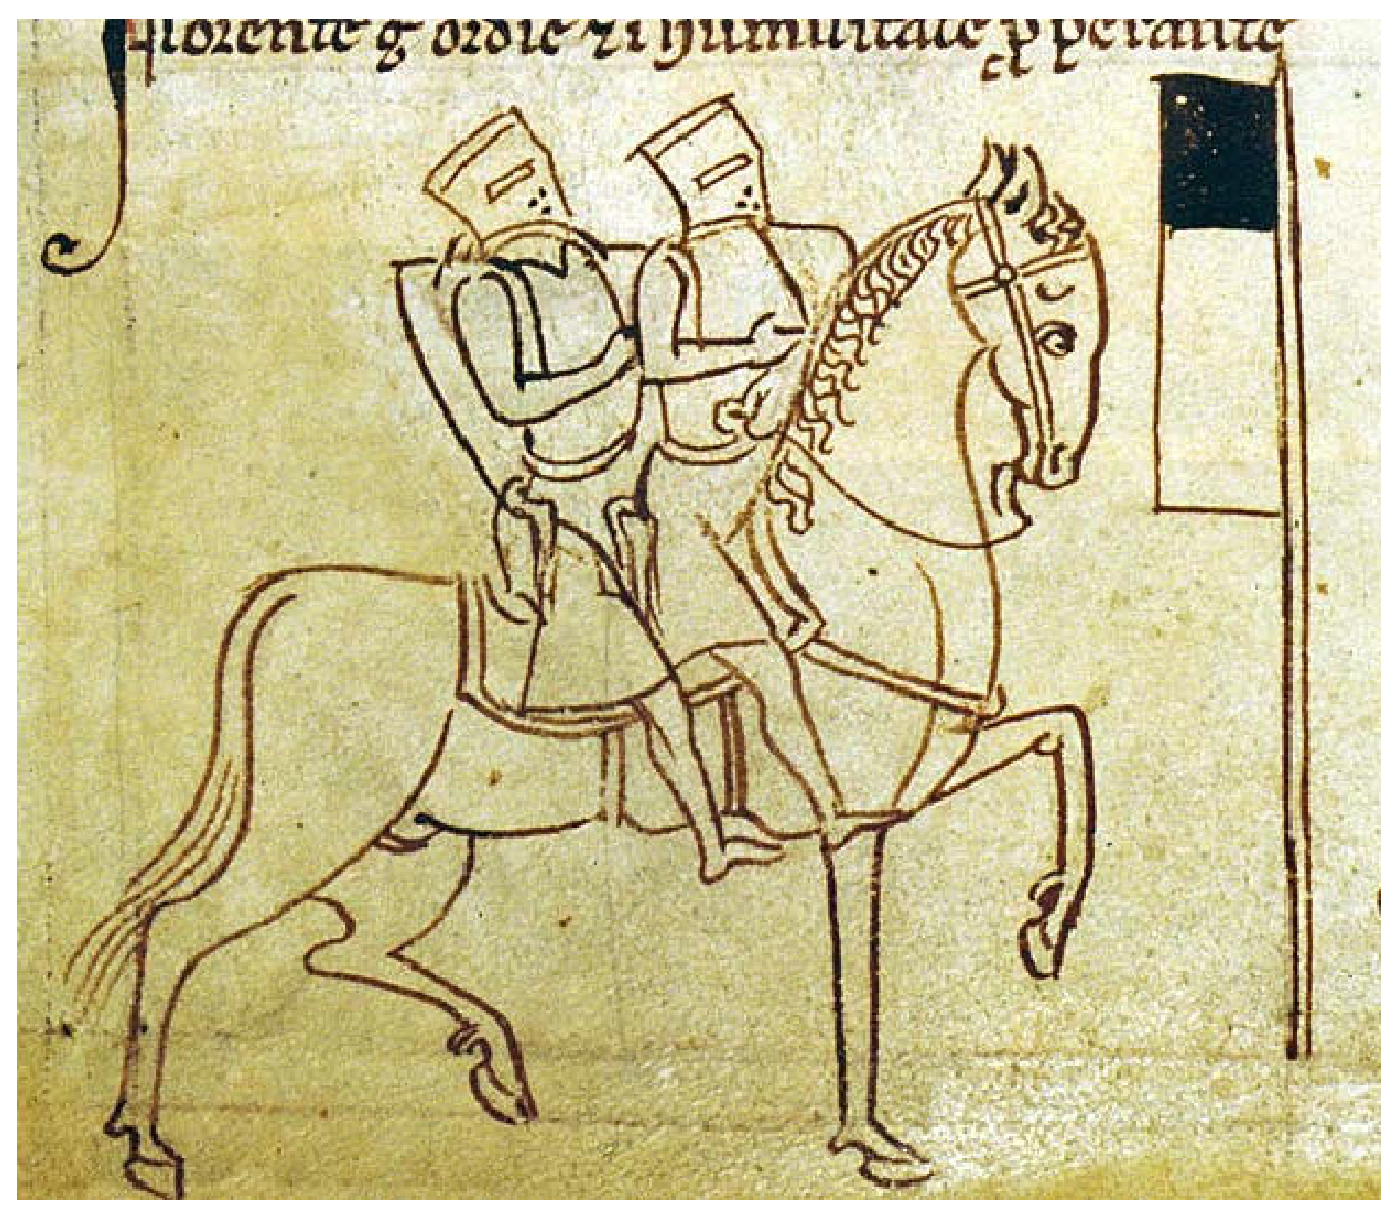
\includegraphics[scale=.4]{templars.eps}
  \end{figure}
\end{frame}
%--------------------------------------

%--------------------------------------
\begin{frame}
 Why are financial intermediaries useful?
\begin{enumerate}
  \item Pooling savings  
  \item Risk diversification
  \item Maturity transformation
  \item Information processing  
\end{enumerate}
\end{frame}
%--------------------------------------

%--------------------------------------
\begin{frame}
 Two types of banking relevant to today's financial system
\begin{enumerate}
  \item Clearing house banks
  \item Fractional reserve banking
\end{enumerate}
\end{frame}
%--------------------------------------

%--------------------------------------
\begin{frame}
  Suppose that one business day the following transactions occur
\begin{itemize}
  \item Bank A: accounts credited with EUR 10M from Bank B depositors
  \item Bank B: credited with EUR 9M from Bank A depositors
\end{itemize}
 \medskip
 Total transfers: EUR 19M\\
 \begin{enumerate}
   \item Have couriers transfer money back and forth
   \item Settle account at end of the business day
 \end{enumerate}
\end{frame}
%--------------------------------------

%--------------------------------------
\begin{frame}
  \textbf{Clearing house bank}
  \begin{itemize}
  \item Will order transfer of EUR 1M from Bank B to Bank A
  \item More efficiently: deduct EUR 1 M from ledger entry for Bank B's account; add it to Bank A's
  \item All deposits still fully backed by the cash in the vaults
\end{itemize}
\medskip
Forerunner of today's central banks
\end{frame}
%--------------------------------------

%--------------------------------------
\begin{frame}
 Most of time only small small fraction of bank's total deposits will be demanded at any given time
 \begin{itemize}
   \item "most" being important qualifier here
 \end{itemize}
 i.e. not all cash has to be in the vault in order to back up the deposits
 \begin{itemize}
   \item Some of it can be used for loans while keeping some cash reserves to deal with day-today demand. 
 \end{itemize}
This practice is called \textbf{fractional reserve banking }
\end{frame}
%--------------------------------------

%--------------------------------------
\begin{frame}
 Some advantages of fractional reserve banking
\begin{enumerate}
  \item Saves depository money: banks can charge interest on loans
  \item Banks serve as an intermediary  
\end{enumerate}
 \medskip
 Disadvantage: risk of bank run
 \begin{itemize}
   \item Assets $\leq$ liabilities (e.g. due to loan defaults)
   \item Suspicion of insolvency could lead depositors to claim their money
 \end{itemize}
 \medskip
 Main issue is a maturity mismatch
 \begin{itemize}
   \item People who supply funds want to have it available for return at shorter terms than the people who the bank lends the money to
 \end{itemize}
\end{frame}
%--------------------------------------

%--------------------------------------
\begin{frame}
 Understanding bank run: bank's balance sheet 
\begin{itemize}
  \item Liabilities: sources of the bank's funds
  \item Assets: uses of said funds
\end{itemize}
\end{frame}
%--------------------------------------

%--------------------------------------
\begin{frame}
 Risky nature of assets
\begin{itemize}
  \item Borrowers don't pay back loans
  \item Bad investments are sometimes made in stocks and bonds
  \item Other assets invested in decline in value
\end{itemize}
\medskip
 Result: negative equity capital
 \begin{itemize}
   \item Assets go below what is owed to depositors and bond-holders
   \item Might trigger bank run when bank is suspected to be insolvent
 \end{itemize}  
\end{frame}
%--------------------------------------

%--------------------------------------
\begin{frame}
 Examples recent bank runs:\\
 \medskip
 2001: Bank run in Argentina during economic crisis (1999-2002)
 2007: Northern Rock, UK\\
 2009: DSB Bank, the Netherlands\\
 2015: Bank runs in Greece and Cyprus
\end{frame}
%--------------------------------------

%--------------------------------------
\begin{frame}
  What happens during a bank run? 
\begin{enumerate}
  \item Banks starts paying off depositors; selling off most liquid assets: e.g. cash, excess reserves at central bank, etc.
  \item Bank sells non-liquid assets: long-term customer loans, property assets: fire sale
\end{enumerate}
 \medskip
 Bank runs often triggered by - assumed- insolvency: makes bank make more insolvent
 \begin{itemize}
   \item Bank run can be triggered by just rumours
   \item Banks and governments are always quick to declare that the banks are fully solvent
   \item Main concern of bank run is contagion risk
 \end{itemize}
\end{frame}
%--------------------------------------

%--------------------------------------
\begin{frame}
\begin{table}[!h] \centering
\caption{Stylised bank balance sheet}
\scalebox{1}{
\begin{tabular}{ll}
\\[-1.8ex]\hline \hline \\[-1.8ex]
    Assets (use of funds)  & Liabilities (source of funds)\\
    \hline \\ 
    Loans & Deposits\\
    Securities & Other borrowings\\
    Cash and reserves  & Equity capital\\
    \\[-1.8ex]\hline \hline \\[-1.8ex]
    \end{tabular}}
\end{table}
\end{frame}
%--------------------------------------

%--------------------------------------
\begin{frame}  
Banking crisis likely leads to credit squeeze
\begin{align*}
  Loans= Deposits + Other\;Borrowings + Equity\;Capital\\
  - Cash\;and\;reserves -   Securities
\end{align*}
\end{frame}
%--------------------------------------

%--------------------------------------
\begin{frame}
  \begin{enumerate}
  \item Loans
  \begin{itemize}
    \item Hard to call in
    \item When paid-off, funds kept as cash, reserves, or invested in securities
    \item Pay off deposit outflows or maturing bond liabilities
    \item Don't make new loans!
  \end{itemize}
  \item Deposits
  \begin{itemize}
    \item Customers prefer cash at home: banks will have less funds to loan
  \end{itemize}
  \item Other borrowings
  \begin{itemize}
    \item Bond markets/other fund providers likely reluctant to lend to banks, worrying they might fail    
  \end{itemize}
  \item Cash and reserves
  \begin{itemize}
    \item Will be kept on balance sheet: needed to survive potential bank run
  \end{itemize}
  \item Securities
  \begin{itemize}
    \item Preferred: can be quickly sold to raise cash
  \end{itemize}
\end{enumerate} 
\end{frame}
%--------------------------------------

%--------------------------------------
\begin{frame}
  Credit crunch result of behaviour of bank and customers
  \begin{itemize}
    \item Bank no longer in position to lend: financial intermediation breaks down
  \end{itemize}
  \medskip
  Banking crisis can lead to severe recession
\end{frame}
%--------------------------------------

%--------------------------------------
\begin{frame}
 Modern banking system has number of features that make crisis difficult to deal with
\begin{itemize}
  \item Non-deposit funding
  \item Interbank linkages
  \item Financial assets and negative feedbacks  
\end{itemize}
\end{frame}
%--------------------------------------

%--------------------------------------
\begin{frame}
 Also, incentive problem
 \begin{itemize}
   \item Bankers moved from risk-averse moneylenders to risk-loving gamblers
 \end{itemize}
\begin{enumerate}
  \item High leverage (little equity capital relative to assets)
  \item Many risky investments
  \item Too much short-term non-deposit funding
  \item Too big
\end{enumerate}
\end{frame}
%--------------------------------------

%--------------------------------------
\begin{frame}
  Imagine investment group starts a bank with starting capital of EUR 10M
\begin{itemize}
  \item EUR 1M spend on retail branch network
  \item Offer 1\% interest rate on deposits: attracts EUR 50M
  \item EUR 50M to make loans: interest rate of 5\%
  \item EUR 9M in cash and reserves
\end{itemize}
\end{frame}
%--------------------------------------

%--------------------------------------
\begin{frame}
\begin{table}[!h] \centering
\caption{Balance sheet}   
\scalebox{.9}{
\begin{tabular}{lclc}
\\[-1.8ex]\hline \hline \\[-1.8ex]
    Assets (use of funds) &~ & Liabilities (source of funds) & ~\\
    \hline \\ 
    Loans                   & 50    & Deposits        & 50\\
    Branch network building & 1     & Equity capital  & 10\\
    Cash and reserves       & 9     & ~               & ~\\[-1.8ex]\\
    Total                   & 60    & ~               & 60\\
    \\[-1.8ex]\hline \hline \\[-1.8ex]
    \end{tabular}}
\end{table}
\end{frame}
%--------------------------------------

%--------------------------------------
\begin{frame}  
\begin{enumerate}
  \item Revenues
    \begin{itemize}
      \item Loan interest: EUR 2.5M
      \item Fees: EUR 1M
    \end{itemize}
  \item Costs
    \begin{itemize}
      \item Deposit interest: EUR 0.5M
      \item Running costs: EUR 1.5M
    \end{itemize}
\end{enumerate}
\begin{table}[!h] \centering
\caption{Income statement}
\scalebox{.9}{
\begin{tabular}{lclc}
\\[-1.8ex]\hline \hline \\[-1.8ex]
    Revenues  &~  & Costs   &~\\
    \hline \\ 
    Interest income & 2.5     & Interest paid & 0.5\\
    Fees            & 1       & Running costs & 1.5\\[-1.8ex]\\
    Total           & 3.5     & ~             & 2\\
    \\[-1.8ex]\hline \hline \\[-1.8ex]
    \end{tabular}}
\end{table}
\end{frame}
%--------------------------------------

%--------------------------------------
\begin{frame}
 Investment: EUR 10M\\
 Profit: EUR 1.5M\\
 Return on Equity
 \begin{align}
   RoE=\frac{1.5}{10}=15\%
 \end{align}
 \medskip
 Time to expand! 
\begin{itemize}
  \item EUR 0.5M paid in dividends
  \item EUR 1M for more loans
  \item EUR 20M in debt securities to raise funds to make additional loans
\end{itemize}
\end{frame}
%--------------------------------------
%--------------------------------------
\begin{frame}
\begin{table}[!h] \centering
\caption{Balance sheet after expanding the business}
\scalebox{.9}{
\begin{tabular}{lclc}
\\[-1.8ex]\hline \hline \\[-1.8ex]
    Assets (use of funds) &~ & Liabilities (source of funds) & ~\\
    \hline \\ 
    Loans                   & 71  & Deposits        & 50\\
    Branch network building & 1   & Equity capital  & 11\\
    Cash and reserves       & 9   & Debt securities & 20\\[-1.8ex]\\
    Total                   & 81  & ~               & 81\\
    \\[-1.8ex]\hline \hline \\[-1.8ex]
    \end{tabular}}
\end{table}
\end{frame}
%--------------------------------------

%--------------------------------------
\begin{frame}
  Goal of bank is to expand business; through making more loans
  \begin{itemize}
    \item Means attracting more risky borrowers: increase in probability that people don't pay back loans
  \end{itemize}
  \medskip
  Suppose that of the 21M in loans, 5M went to a real estate developer who went bankrupt
\end{frame}
%--------------------------------------


%--------------------------------------
\begin{frame}
\begin{table}[!h] \centering
\caption{Balance sheet after expanding the business}
\scalebox{.9}{
\begin{tabular}{lclc}
\\[-1.8ex]\hline \hline \\[-1.8ex]
    Assets (use of funds) &~ & Liabilities (source of funds) & ~\\
    \hline \\ 
    Loans                   & 66  & Deposits        & 50\\
    Branch network building & 1   & Equity capital  & 6\\
    Cash and reserves       & 9   & Debt securities & 20\\[-1.8ex]\\
    Total                   & 76  & ~               & 76\\
    \\[-1.8ex]\hline \hline \\[-1.8ex]
    \end{tabular}}
\end{table}

\end{frame}
%--------------------------------------

%--------------------------------------
\begin{frame} 
\begin{enumerate}
  \item Equity capital is risky; one bad loan removes a fair chunk
  \item Investors will get paid dividends when there is a profit, but they are the first to lose money when there is a bad loan
  \item Depositors and debt-holders have first claim to getting their money back
\end{enumerate}
 \medskip
  Bank needs to be cautious in assessing credit risk of loan
\end{frame}
%--------------------------------------

%--------------------------------------
\begin{frame}
 Does size matter?\\
 \medskip
 Start bank with equity capital of EUR 10M 
 \begin{itemize}
  \item Pay 2\% on deposits
  \item Charge 3\% on loans
  \item 10\% of deposits reserve requirements 
\end{itemize}
\end{frame}
%--------------------------------------

%--------------------------------------
\begin{frame}
  Consider two approaches to raising funds  
\begin{enumerate}
  \item Conservative 
  \begin{itemize}
    \item  90M raised in deposits
  \end{itemize} 
 \item Aggressive 
  \begin{itemize}
    \item 90M raised in deposits
    \item 1000M borrowed from international money markets (2\% interest rate)
  \end{itemize}
\end{enumerate}
\end{frame}
%--------------------------------------

%--------------------------------------
\begin{frame}
\begin{table}[!h] \centering
\label{table:conservative}
\caption{Balance sheet starting with EUR 100 million}
\scalebox{.9}{
\begin{tabular}{lclc}
\\[-1.8ex]\hline \hline \\[-1.8ex]
    Assets (use of funds) &~ & Liabilities (source of funds) & ~\\
    \hline \\ 
    Loans                   & 91  & Deposits        & 90\\
    Cash and reserves       & 9   & Equity capital  & 10\\[-1.8ex]\\
    Total                   & 100 & ~               & 100\\
    \\[-1.8ex]\hline \hline \\[-1.8ex]
    \end{tabular}}
\end{table}

\begin{table}[!h] \centering
\label{table:aggressive}
\caption{Balance sheet starting with EUR 200 million}
\scalebox{.9}{
\begin{tabular}{lclc}
\\[-1.8ex]\hline \hline \\[-1.8ex]
    Assets (use of funds) &~ & Liabilities (source of funds) & ~\\
    \hline \\ 
    Loans                   & 191  & Deposits        & 90\\
    Cash and reserves       & 9    & Equity capital  & 10\\
    ~                       & ~    & Borrowings      & 100\\[-1.8ex]\\
    Total                   & 200  & ~               & 200\\
    \\[-1.8ex]\hline \hline \\[-1.8ex]
    \end{tabular}}
\end{table}
\end{frame}
%--------------------------------------


%--------------------------------------
\begin{frame}
  Profits and RoE for conservative approach  
\begin{align*}
  \Pi &= 3\%*91 - 2\%*90 = 2.73   - 1.8 =0.93\\
  RoE &= 9.3\%
\end{align*}
\medskip
Profits and RoE for aggressive approach
\begin{align*}
  \Pi &= 3\%*191 - 2\%*190 = 5.73    - 3.82 =1.91\\
  RoE &=19.1\%
\end{align*}
\end{frame}
%--------------------------------------

%--------------------------------------
\begin{frame}
  Larger bank has 
  \begin{itemize}
    \item Lower capital-to-assets ratio
    \item Higher profits
    \item Higher RoE
  \end{itemize}
  \medskip
  Highly-leverage banks make larger profits but also take more risks
  \begin{itemize}
    \item More credit risk since loans could go bad, 
    \item More liquidity risk as funds from international money market could dry up
  \end{itemize}
  \medskip
  Not in banker's self-interest to maintain sufficient capital levels\\
  \medskip
  \textbf{Leverage ratio} is the assets-capital ratio
\begin{enumerate}
  \item Small bank: 10: equity capital was 10\% of total assets 
  \item Large bank: 20  equity capital was 5\% of total assets 
\end{enumerate}
\end{frame}
%--------------------------------------

%--------------------------------------
\begin{frame}
 Two sets of incentives  
\begin{enumerate}
  \item Investors
  \begin{itemize}
    \item Shareholders of highly-leveraged banks willing to lose all their money with prospect of high returns most of the time
    \item When things go pear-shaped, may have made a decent enough return from all the dividends
  \end{itemize}
  \item Bank management
  \begin{itemize}
    \item Even when investors are risk adverse there are strong incentives for high leverage
    \item E.g. profit-linked bonuses, which means that they want to maximise profit today
    \item In case of bankruptcy don't have to pay back bonuses
    \item Government bailout: privatised profits, socialised losses 
  \end{itemize}
\end{enumerate}
\end{frame}
%--------------------------------------

%--------------------------------------
\begin{frame} 
  \textbf{Value at Risk}, measure for risk level of investments of a bank, motivated by question
  \begin{quote}
    What is, realistically, the worst that could happen over one day, one week, ore one year?
  \end{quote}
  \begin{align}
    Pr(W<W_0-VaR)\leq 1-\alpha
  \end{align}
  \begin{align}
    VaR \equiv inf\{V|F(W_0-V)\leq1-\alpha\}
  \end{align}
\end{frame}
%--------------------------------------

%--------------------------------------
\begin{frame}
  \begin{figure}
    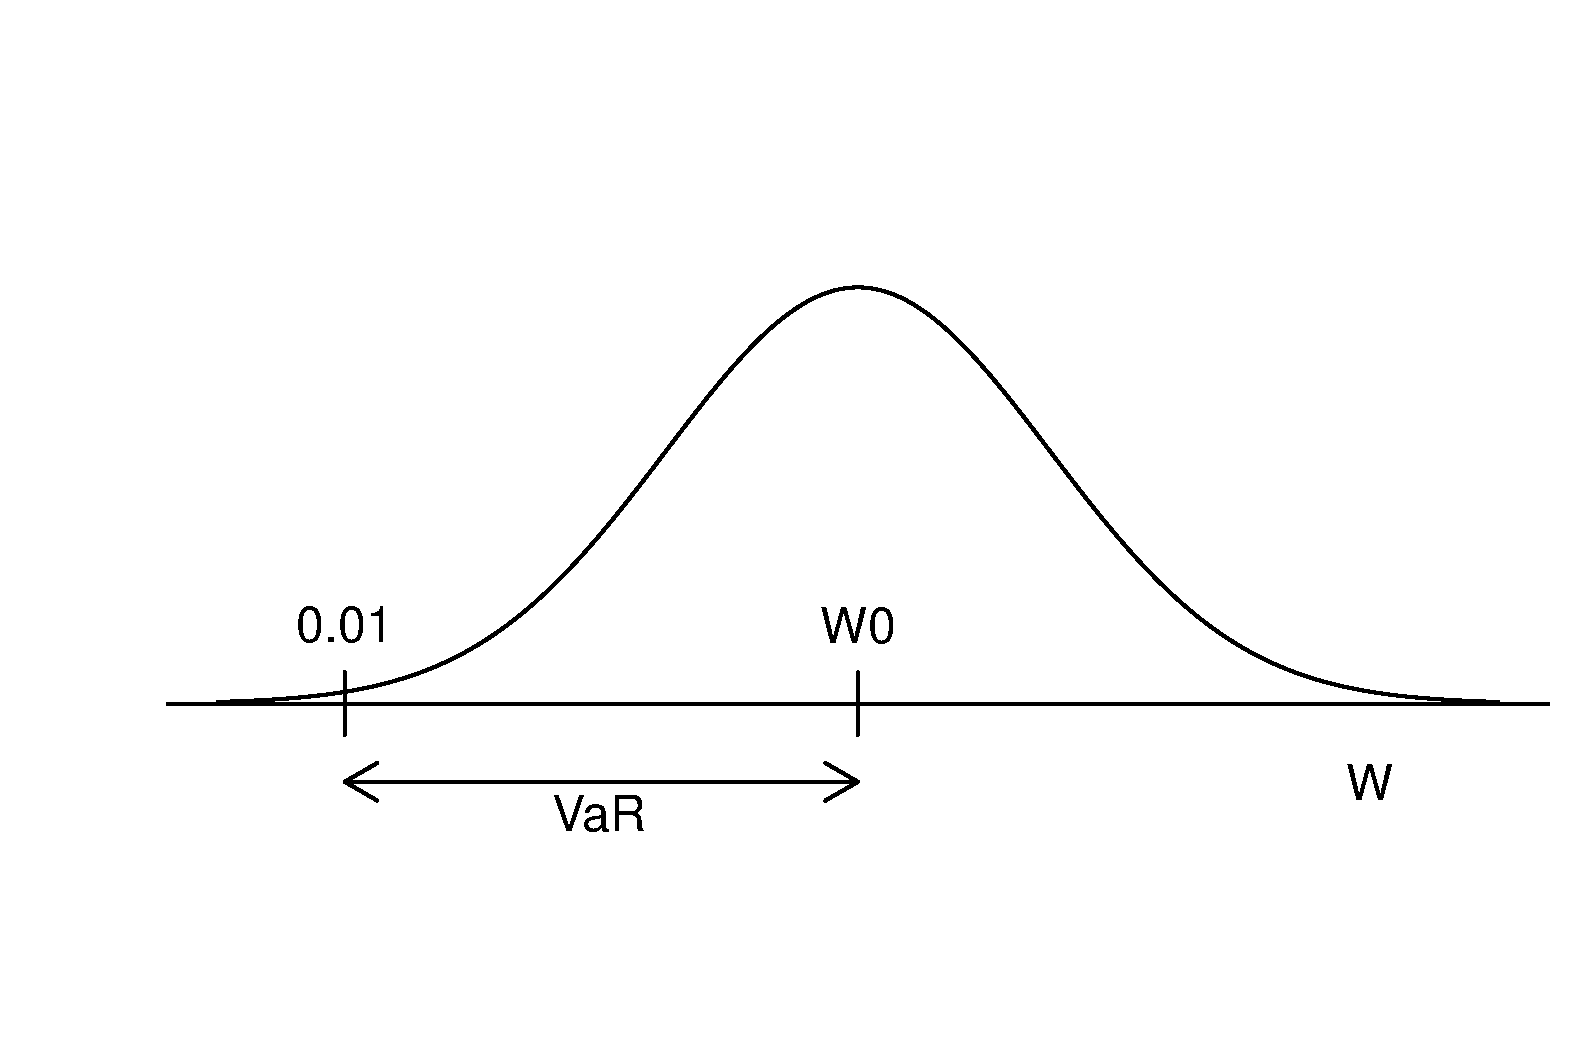
\includegraphics[scale=.3]{VaR.eps}
  \end{figure}
\end{frame}
%--------------------------------------


%--------------------------------------
\begin{frame}
  VaR estimates possible loss under normal market conditions, using statistical distribution of the bank's credit losses
\begin{itemize}
  \item Expected loss (distribution average) 
  \begin{itemize}
    \item Banks should deal with these by writing down part of their loans each year as loan loss provision
    \item i.e. valuing assets at less than their current book value in anticipation of future losses
  \end{itemize}
  \item Stress loss (distribution extreme tail)
  \begin{itemize}
    \item 1\% tail is commonly used
    \item e.g. at a weekly VaR of EUR 50 million, there is  1\% chance that your portfolio will lose more than EUR 50 million over the course of a week 
  \end{itemize}
\end{itemize}
\end{frame}
%--------------------------------------

%--------------------------------------
\begin{frame} 
  A bank is owed money by two firms
  \begin{itemize}
    \item 1M by firm A, 1M by firm B
  \end{itemize}
  Both firms are credit worthy and pay back the loan with $Pr=0.995$
  \begin{itemize}
    \item When A defaults, bank can recover 0.5M
    \item When B defaults, nothing can be recovered
  \end{itemize}
  \begin{align}
    VaR=0
  \end{align}
\end{frame}
%--------------------------------------

%--------------------------------------
\begin{frame}
 \begin{align}
   Pr(repayment < 1M-x)\leq 0.01
 \end{align}
 Both firms repay with $Pr=0.995$; can set $x=0$
 \begin{align}
   Pr(repayment < 1M)=0.005 \leq 0.01
 \end{align}
 However, banks has more to lose when firm B defaults; need better measure.
 \begin{align}
    Tail\;loss = \mathbb{E}(W|W<q) = \frac{\int^q_{-\infty}Wf(W)dW}{\int^q_{-\infty}f(W)dW}
  \end{align}
\end{frame}
%--------------------------------------

%--------------------------------------
\begin{frame}
  \begin{figure}
    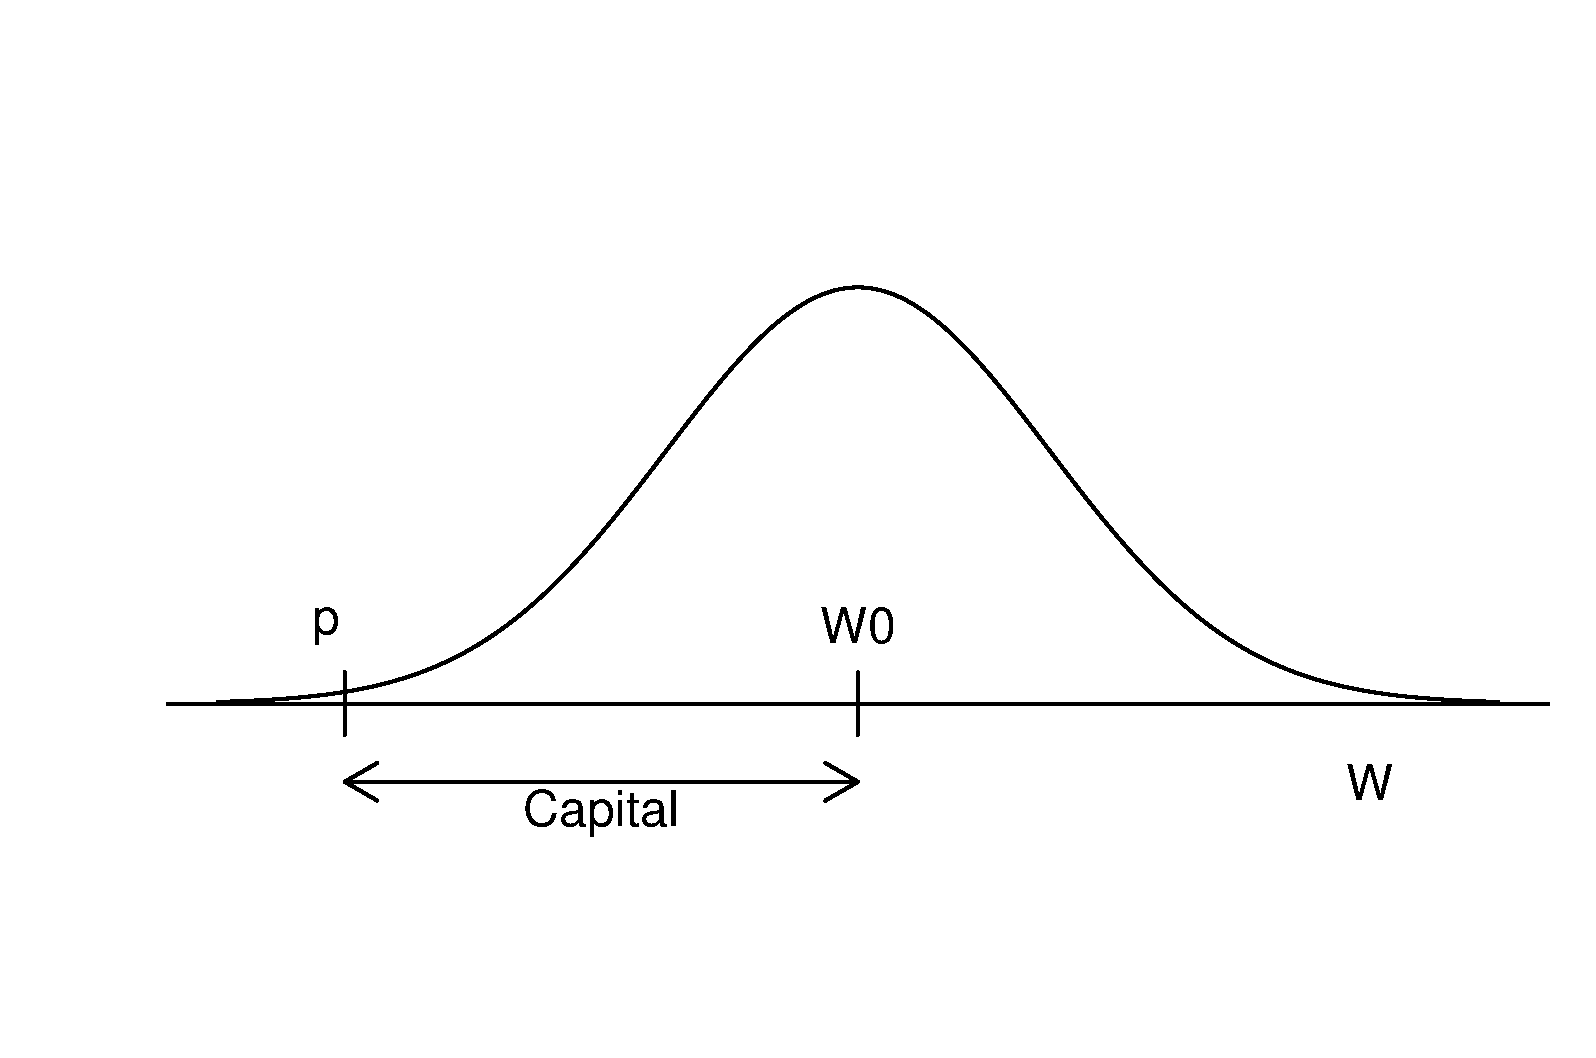
\includegraphics[scale=.3]{VaR2.eps}
  \end{figure}
\end{frame}
%--------------------------------------

%--------------------------------------
\begin{frame}
  Bank will go bankrupt with probability $p$
  \begin{itemize}
    \item Failure probability can be decreased by holding more capital
    \item VaR indicates amount of capital required to stave off default with high probability
  \end{itemize}
  \medskip
  Tail loss no concern for equity holders
  \begin{itemize}
    \item Is of interest to creditors and other actors in wider economy; these do not control the bank
  \end{itemize}
\end{frame}
%--------------------------------------

%--------------------------------------
\begin{frame}
  Time horizon in VaR should be long enough so that
  \begin{itemize}
    \item Corrective measures can be taken to rectify problem
    \item Horizon is appropriate for degree of asset illiquidity
    \item Uncertainty level chosen to account for ease of recapitalisation
  \end{itemize}
\end{frame}


%--------------------------------------
\begin{frame}
 VaR bedrock of capital regulations by Basel regulations
  \begin{itemize}
    \item Minimum level regulatory capital equal to some multiple of unexpected losses
    \begin{align*}
      Capital\; Required = 3\cdot VaR
    \end{align*}
  \end{itemize}
   Basel regulations also require risk-weighted assets of $\geq$8\%
\begin{align*} 
  RWA=\frac{3*VaR}{0.08} 
\end{align*}

\end{frame}
%--------------------------------------

%--------------------------------------
\begin{frame}
  Final RWA figure determined by some adjustments
  \begin{enumerate}
    \item Market risk
    \begin{quote}
      pertaining to interest rate related instruments, equities, foreign exchange risk and commodities risk
    \end{quote}
    \item Operational risk
    \begin{quote}
      inadequate or failed internal processes, people and systems or from external events
    \end{quote}
  \end{enumerate}
\end{frame}
%--------------------------------------

%--------------------------------------
\begin{frame}
 VaR shortcoming: uses distribution of past asset returns 
\begin{enumerate}
  \item Estimation sample
  \begin{itemize}
    \item True distribution not known; can only be estimated from historical data
    \item Banks rely mainly on using returns from recent years
  \end{itemize}
  \medskip
  \item Tail risk
  \begin{itemize}
    \item Fat tails not accounted for
    \item Financial markets generate extreme losses more often than predicted by normal distribution    
  \end{itemize}
\end{enumerate}
\end{frame}
%--------------------------------------

%--------------------------------------
\begin{frame}
  Interbank markets can help banks coping with reserve requirements
\begin{itemize}
  \item Lending and borrowing short-term funds
  \item Allowing banks with lots of deposits but without good loan opportunities to lend to banks with good loan opportunities but limited deposits
\end{itemize}
\medskip
Despite advantage, interbank lending can make system unstable
\end{frame}
%--------------------------------------

%--------------------------------------
\begin{frame}
 Consider three banks ($A,B,C$), each with a equity capital of EUR 10M\footnote{Note that this example is not entirely realistic as the amount of capital lost by the first bank is greater than the total amount of capital in the system.}  
 \begin{enumerate}
   \item A borrows EUR 25M from B
   \item B borrows EUR 15M from C 
 \end{enumerate}
 \medskip
 A loses EUR 35M in loans: wipes out equity capital
\begin{enumerate}
  \item Bank A loses 
  \item A becomes insolvent $\rightarrow$ B loses EUR 25M
  \item B becomes insolvent $\rightarrow$ cannot pay C
  \item C becomes insolvent and has no equity capital left
\end{enumerate}
Insolvency of one bank can bring down whole system: \textbf{systemic risk}
\end{frame}
%--------------------------------------

%--------------------------------------
\begin{frame}
  Single bank can pose risk for whole financial system through  
\begin{enumerate}
  \item Contagion (interbank lending)
  \item Spillovers (asset sales)
  \begin{itemize}
    \item Troubled bank sells liquid assets
    \item Fire sale puts downward pressure on asset price
    \item Due to regulation asset value other banks marked down
    \item Fire sale reduces equity capital $\rightarrow$ increasing risk other banks
  \end{itemize}
\end{enumerate}
\end{frame}
%--------------------------------------

%--------------------------------------
\begin{frame}
  \textbf{Alessandri \& Haldane}(2009) "Banking on the state"
\begin{itemize}
  \item The banking sector has grown in size relative to the economy
  \item Banks have become more leveraged and less liquid
  \item Have engaged in more risky trading activities
\end{itemize}
 \begin{figure}
   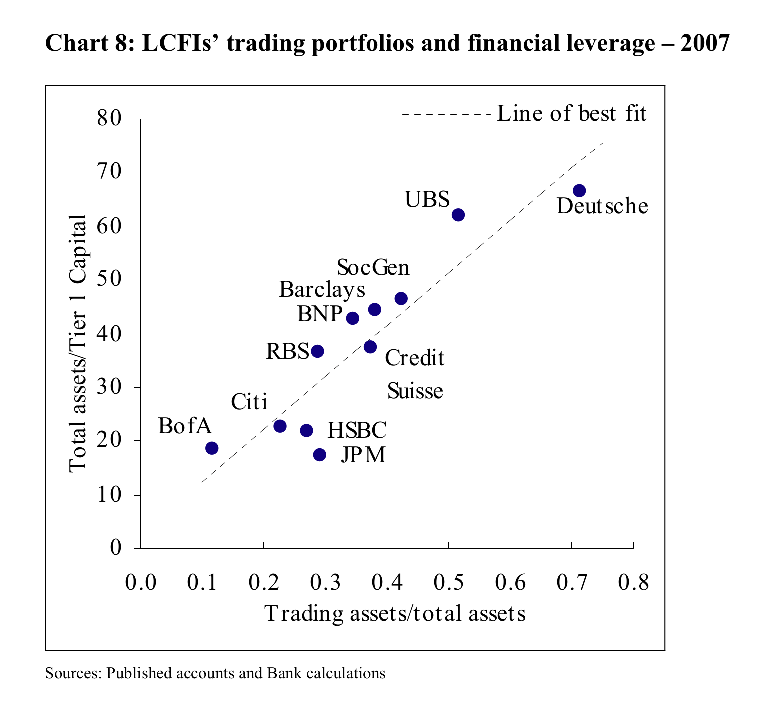
\includegraphics[scale=.4]{bank_state.eps}
 \end{figure}
\end{frame}
%--------------------------------------

%--------------------------------------
\begin{frame}
 \textbf{Prudential regulation} can lead to financial instability
  \begin{enumerate}
  \item Asset prices increase during boom, loans paid back: increase in equity
  \item Can expand operation: acquire new assets; liquidity not issue with large demand: boom continues
  \item Boom turns into bust: business cycle plays out; recession arrives
  \item Capital requirement will lead to asset sell off: price decrease will erode equity
\end{enumerate}
\end{frame}
%--------------------------------------

%--------------------------------------
\begin{frame}
  \textbf{Power law}
  \begin{align}
    f(x)=Ax^{-\alpha}
  \end{align}
  \medskip
  $\alpha$, scaling parameter\\
  $A$, constant
\end{frame}
%--------------------------------------

%--------------------------------------
\begin{frame}
 \textbf{Barro \& Jin} (2011) "On the size distribution of macroeconomic disasters"
 \begin{align}
   log(Y_{t+1}) &= log(Y_t)+g+u_{t+1}+v_{t+1}\\ \nonumber
   Y_t&=C_t; g \geq 0 \\
 \end{align}
 $v_{t+1}$ accounts for low-probability disasters: output contracts by fraction $b$
 \begin{align}
   0 < b \leq 1
 \end{align}
 \begin{align}
   Pr(1-p) &: v_{t+1}=0\\ \nonumber
   Pr(p) &: v_{t+1} =log(1-b)
 \end{align}
 \begin{align}
   g^* &= g+ \frac{1}{2}\cdot\sigma^2 -p\cdot Eb
 \end{align}
\end{frame}
%--------------------------------------

%--------------------------------------
\begin{frame}
  Disaster size
  \begin{align}
    z &\equiv 1/(1-b)
  \end{align}
  \medskip
  Single power law
  \begin{align}
    f(z) &= Az^{-(\alpha+1)}\\
    A&=\alpha z_0^{\alpha}    
  \end{align}
  \medskip
  Double power law
  \begin{align}
    f(z) = \begin{Bmatrix}
      0, & if\; z<z_0,\\
      Bz^{-(\beta+1)}, & if\; z_0 \leq z \leq \delta,\\
      Az^{-(\alpha+1)}, &if\; \delta \leq z, 
    \end{Bmatrix}
  \end{align}
\end{frame}
%--------------------------------------

%--------------------------------------
\begin{frame}
  \begin{figure}
    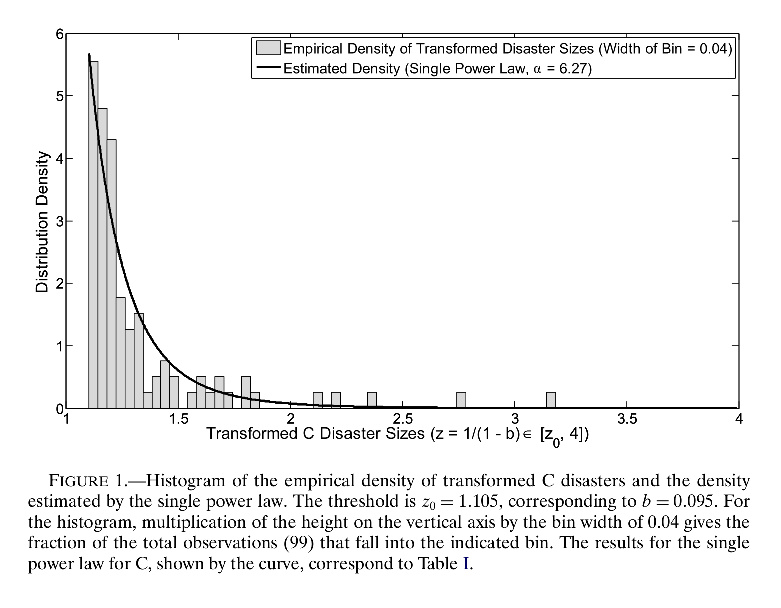
\includegraphics[scale=.7]{barro_jin1.eps}
  \end{figure}
\end{frame}
%--------------------------------------

%--------------------------------------
\begin{frame}
  \begin{figure}
    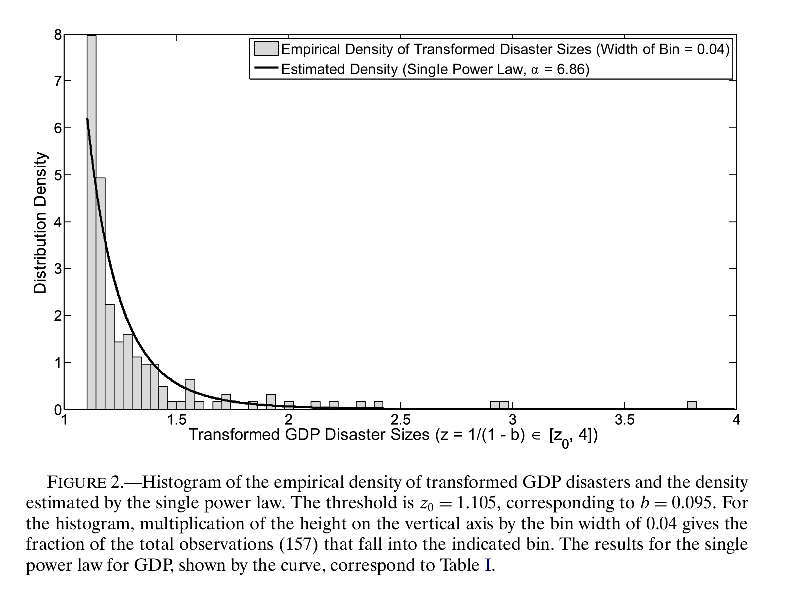
\includegraphics[scale=.7]{barro_jin2.eps}
  \end{figure}
\end{frame}
%--------------------------------------

%--------------------------------------
\begin{frame}
  \begin{figure}
    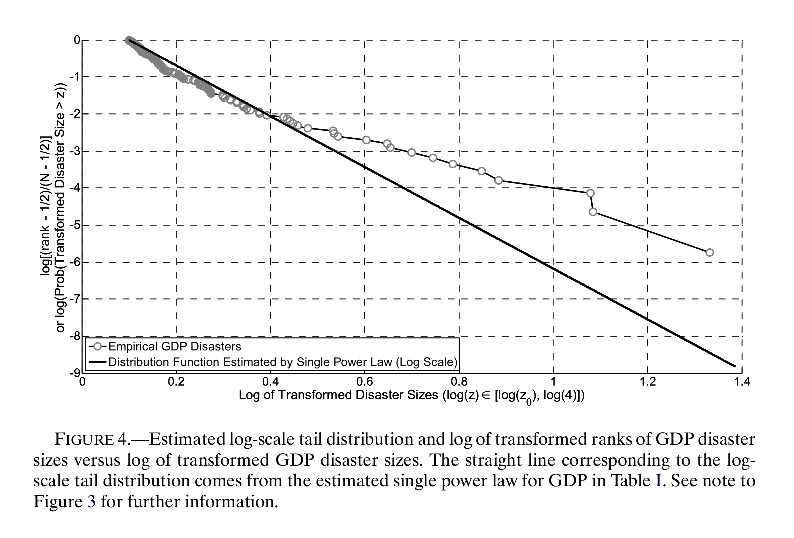
\includegraphics[scale=.7]{barro_jin3.eps}
  \end{figure}
\end{frame}
%--------------------------------------

%--------------------------------------
\begin{frame}
  \begin{figure}
    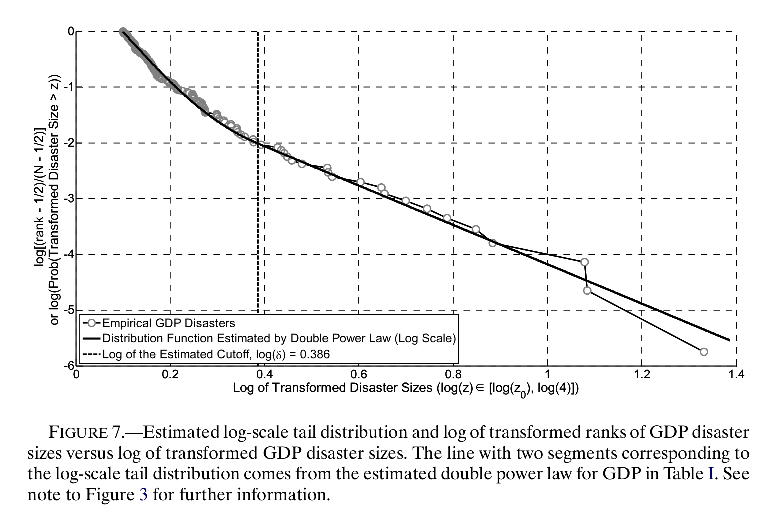
\includegraphics[scale=.7]{barro_jin4.eps}
  \end{figure}
\end{frame}
%--------------------------------------


%--------------------------------------
\begin{frame}
 \textbf{Gourio} (2012) "Disaster risk and business cycles"\\
 \medskip
 Normal times
 \begin{align}
   log\;z_{p,t}&= log\; z_{p,t-1} + \mu + \epsilon_t \\
   log\; z_{r,t} &= \rho_z log\; z_{r,t-1}
 \end{align}
 \medskip
 Disasters
  \begin{align}
    K_{t+1} &= \left( (1-\delta)K_t + \phi \left(\frac{I_t}{K_t}\right)K_t e^{\zeta_{t+1}} \right)\\
    log\;z_{p,t}&= log\; z_{p,t-1} + \mu + \epsilon_t + \theta_t \\
    log\; z_{r,t} &= \rho_z log\; z_{r,t-1} +\varphi_t - \theta_t\\
    log(p_t) &= \rho_p log(p_{t-1}) + (1-\rho_p)log\overline(p)+\epsilon_t^p
  \end{align}
  \begin{align}
   Pr(x_{t+1}=1 | x_t=1) &= max(q,p_t)\\
   Pr(x_{t+1}=1 | x_t=0) &= p_t
 \end{align}
\end{frame}
%--------------------------------------

%--------------------------------------
\begin{frame}
  \begin{figure}
    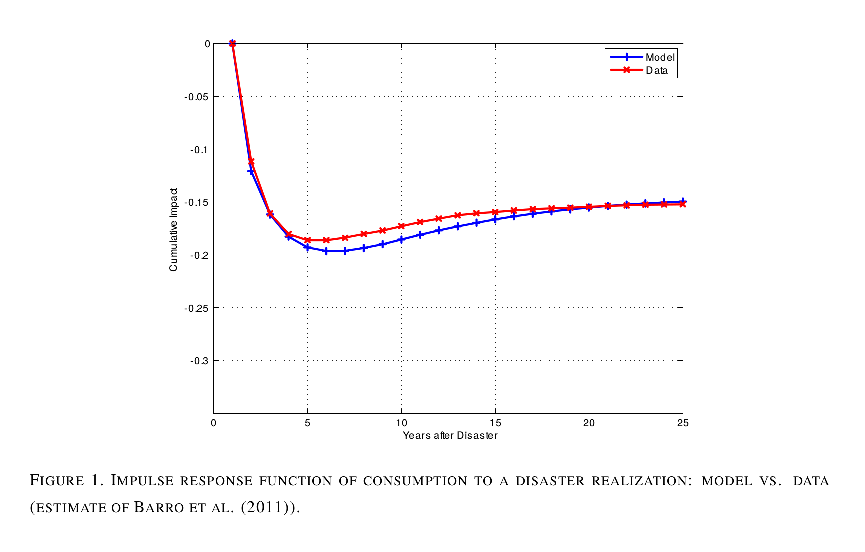
\includegraphics[scale=.8]{gourio1.eps}
  \end{figure}
\end{frame}
%--------------------------------------

%--------------------------------------
\begin{frame}
\begin{figure}
    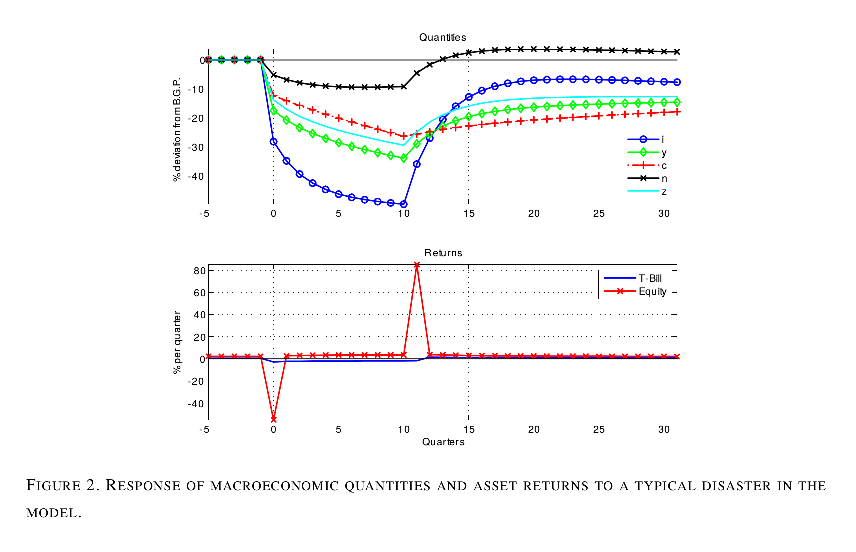
\includegraphics[scale=.8]{gourio2.eps}
  \end{figure}
\end{frame}
%--------------------------------------

%--------------------------------------
\begin{frame}
\begin{figure}
    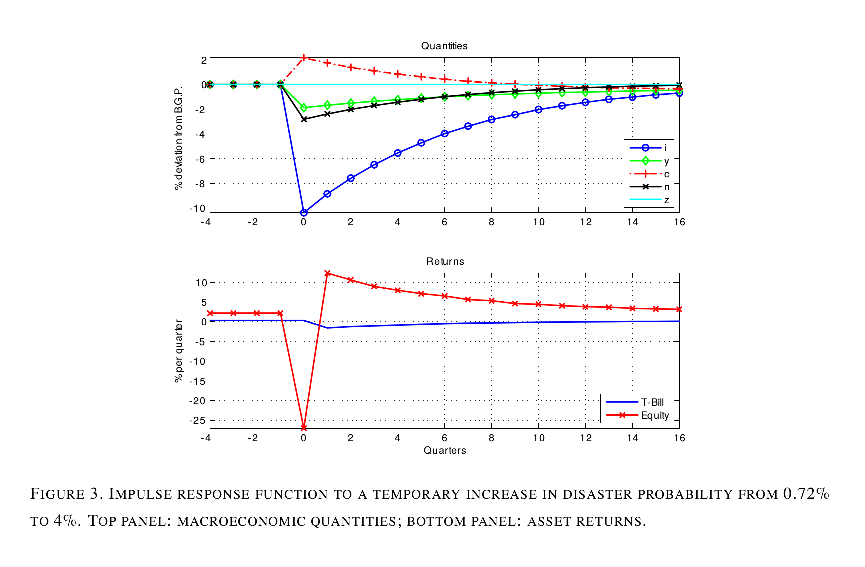
\includegraphics[scale=.8]{gourio3.eps}
  \end{figure}
\end{frame}
%--------------------------------------

%--------------------------------------
\begin{frame}
  \textbf{Boissay et al.} (2016) "Booms and Banking Crises"\\ 
  \medskip
  Financial recessions are sui generis
  \begin{enumerate}
    \item They are rare events
    \item Are deeper and last longer compared to other recessions
    \item Follow credit booms (i.e. not random)
  \end{enumerate}
  \medskip
  Model: bank heterogeneity leads to interbank market
  \begin{itemize}
    \item Moral hazard and asymmetric information may lead eventually to financial recession
  \end{itemize}
  \medskip
  Illustrate that these recession are not triggered by adverse exogenous shocks
  \begin{align}
    P(z_{t+1}<\overline{z}_{t+1}|z_t,A_t) = \Phi(log \overline{z}_{t+1}-\rho_zlog z_t)
  \end{align}
\end{frame}
%--------------------------------------

%--------------------------------------
\begin{frame}
  \begin{figure}
    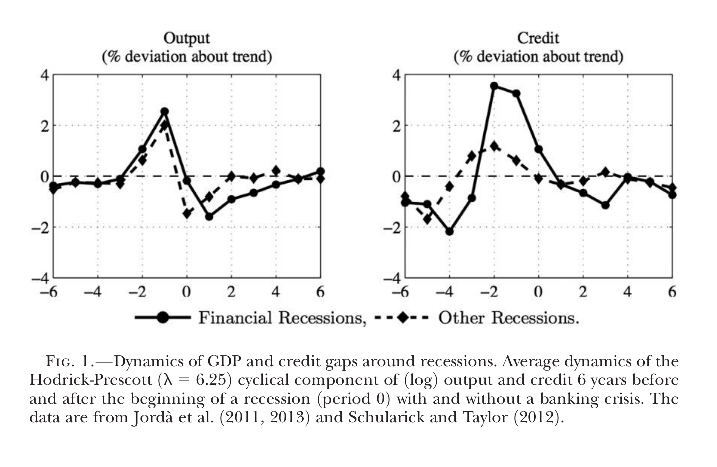
\includegraphics[scale=.7]{boissay.eps}
  \end{figure}
\end{frame}
%--------------------------------------

%--------------------------------------
\begin{frame}
  \begin{figure}
    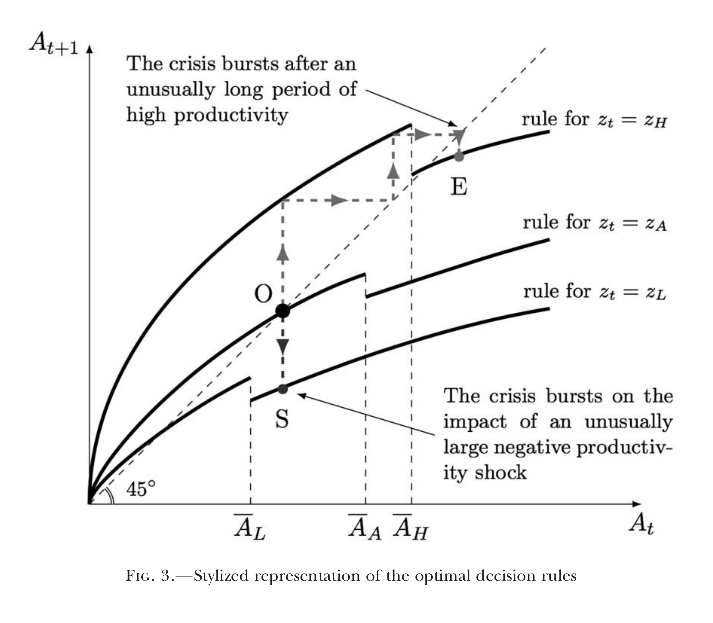
\includegraphics[scale=.7]{boissay2.eps}
  \end{figure}
\end{frame}
%--------------------------------------

%--------------------------------------
\begin{frame}
  \begin{figure}
    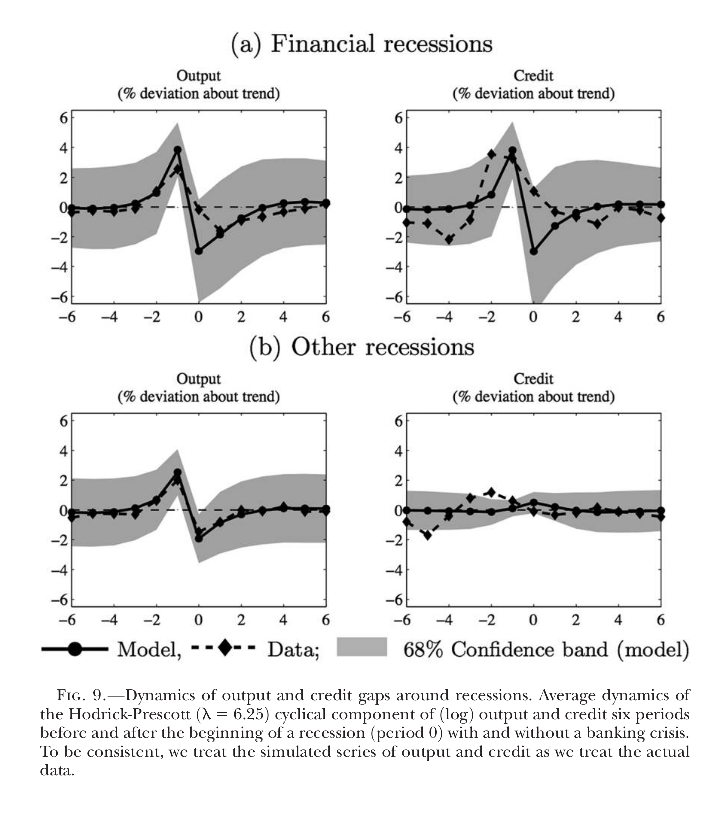
\includegraphics[scale=.7]{boissay3.eps}
  \end{figure}
\end{frame}
%--------------------------------------

%--------------------------------------
\end{document}
